\documentclass[conference]{IEEEtran}
\IEEEoverridecommandlockouts

\usepackage{cite}
\usepackage{amsmath,amssymb,amsfonts}
\usepackage{graphicx}
\usepackage{textcomp}
\usepackage{xcolor}
\usepackage{array}
\usepackage{url}
\usepackage{tikz}
\usetikzlibrary{arrows.meta,positioning}
\usepackage{booktabs}
\usepackage{multirow}
\usepackage{listings}
\usepackage{xcolor}

\lstset{
	basicstyle=\ttfamily\footnotesize,
	breaklines=true,
	frame=single,
	numbers=left,
	numberstyle=\tiny,
	captionpos=b,
	showstringspaces=false,
	tabsize=2
}

% ============================================================
% FLOAT CONTROL (NO stfloats / NO dblfloatfix)
% ============================================================
\usepackage[section]{placeins} % prevents floats crossing sections
\usepackage{float}             % provides [H] for "exactly here" (use mainly in appendix)

% Encourage floats to stay close to where they are written
\renewcommand{\topfraction}{0.95}
\renewcommand{\bottomfraction}{0.95}
\renewcommand{\textfraction}{0.05}
\renewcommand{\floatpagefraction}{0.90}
\setcounter{topnumber}{2}
\setcounter{bottomnumber}{2}
\setcounter{totalnumber}{4}

% Make LaTeX less eager to float everything away
\setlength{\textfloatsep}{8pt plus 2pt minus 2pt}
\setlength{\floatsep}{6pt plus 2pt minus 2pt}
\setlength{\intextsep}{6pt plus 2pt minus 2pt}

\def\BibTeX{{\rm B\kern-.05em{\sc i\kern-.025em b}\kern-.08em
		T\kern-.1667em\lower.7ex\hbox{E}\kern-.125emX}}

% ============================================================
% Paths (relative to Report/)
% ============================================================
\newcommand{\RUNROOT}{../Code/runs_20251213_101931}
\newcommand{\MAINRUN}{dep2030-01-01_2032-01-01_arr2030-05-01_2032-12-26}
\newcommand{\PLOT}[2]{\RUNROOT/#1/plots/#2}

% ============================================================
% Safe include (placeholder if missing)
% ============================================================
\makeatletter
\newcommand{\safeincludegraphics}[2][]{%
	\begingroup
	\edef\@tmp{#2}%
	\edef\@figpath{\detokenize\expandafter{\@tmp}}%
	\IfFileExists{\@figpath}{%
		\includegraphics[#1]{\@figpath}%
	}{%
		\fbox{\parbox{0.95\linewidth}{\centering
				\vspace{0.06\textheight}
				\textbf{Missing figure}\\[0.4em]
				\small\texttt{\@figpath}
				\vspace{0.06\textheight}
		}}%
	}%
	\endgroup
}
\makeatother

% ============================================================
% Figure helpers: main = column width, backup = full page width
% ============================================================
\newcommand{\FIGCOL}[1]{\safeincludegraphics[width=\columnwidth]{#1}}
\newcommand{\FIGFULL}[1]{\safeincludegraphics[width=\textwidth]{#1}}

\begin{document}
	
	\title{Data-Driven Approximation of Earth--Mars Pork-Chop Surfaces Using Neural-Network Surrogates}
	
	\author{\IEEEauthorblockN{Scott Nguyen}
		\IEEEauthorblockA{\textit{Dept. of Electrical and Computer Engineering}\\
			\textit{University of New Mexico}\\
			Albuquerque, NM, USA}}
	\maketitle
	
	% ============================================================
	\begin{abstract}
		Interplanetary mission design requires repeated evaluation of transfer costs across large launch windows, typically performed by solving Lambert’s problem at thousands of grid points to construct pork-chop plots. While accurate, brute-force Lambert sweeps are computationally expensive and limit rapid trade-space exploration or repeated optimization. This paper presents a data-driven surrogate modeling approach to approximate Earth--Mars pork-chop surfaces by mapping departure epoch and time-of-flight to total $\Delta V$. For each of five two-year windows spanning 2030--2040, Lambert solutions are generated on a dense grid and filtered by a feasibility threshold of $\Delta V \le 20$~km/s. A compact multi-layer perceptron (MLP) is trained on valid samples only and evaluated using MAE, RMSE, and $R^2$ on held-out data. In early windows, the surrogate achieves sub-1~km/s MAE and reproduces the dominant low-energy corridors of the Lambert surface. Later windows exhibit larger generalization error and can produce spurious surrogate optima, emphasizing the need for feasibility-aware constraints and validation against the true objective.
	\end{abstract}
	
	\begin{IEEEkeywords}
		interplanetary trajectory design, pork-chop plots, surrogate modeling, Lambert problem, Earth--Mars transfer, neural networks
	\end{IEEEkeywords}
	
	% ============================================================
	\section{Introduction}
	Interplanetary trajectory design explores trade spaces defined by departure epoch, time-of-flight (TOF), and total velocity increment $\Delta V$. Pork-chop plots visualize $\Delta V(t_{\mathrm{dep}},\mathrm{TOF})$ and reveal low-energy corridors for candidate launch opportunities. Constructing these surfaces via Lambert sweeps requires solving Lambert’s problem at every grid point, which becomes expensive for wide windows or repeated optimization.
	
	Machine learning can reduce repeated computation via surrogate models that approximate expensive physics-based objectives. Surrogate neural networks have accelerated simulation-based optimization loops by replacing repeated forward calls with fast regressors~\cite{ruff2023}. Reinforcement learning and meta-RL have also been explored for robust trajectory design under uncertainty~\cite{zavoli2021,federici2024}. This work focuses on supervised learning for impulsive Earth--Mars Lambert pork-chop approximation.
	
	\subsection{Contributions}
	\begin{itemize}
		\item A reproducible pipeline for generating Earth--Mars Lambert datasets across five two-year windows from 2030 to 2040.
		\item A compact MLP surrogate for $\Delta V$ prediction from $(t_{\mathrm{dep}}, \mathrm{TOF})$.
		\item Quantitative and qualitative assessment of surrogate fidelity and optimization behavior across windows.
	\end{itemize}
	
	% ============================================================
	\section{Background}
	Lambert’s problem provides an impulsive two-body approximation for connecting heliocentric endpoints in a fixed time. Sweeping departure date and TOF yields pork-chop surfaces whose valleys correspond to favorable geometries. Data-driven surrogates aim to approximate these surfaces with orders-of-magnitude lower evaluation cost. Prior work demonstrated surrogate networks in simulation-based optimization~\cite{ruff2023} and learning-based robust trajectory methods~\cite{zavoli2021,federici2024}. The present study isolates the supervised surrogate approximation problem for impulsive Earth--Mars transfers.
	
	% ============================================================
	\section{Objective and Problem Formulation}
	\subsection{Two-Body Transfer Model}
	We assume heliocentric two-body dynamics during the transfer arc:
	\begin{equation}
		\ddot{\mathbf{r}}(t) = -\mu_{\odot}\frac{\mathbf{r}(t)}{\|\mathbf{r}(t)\|^3}.
		\label{eq:twobody}
	\end{equation}
	Decision variables are the departure epoch and TOF:
	\begin{equation}
		x \triangleq \begin{bmatrix} t_{\mathrm{dep}} \\ \mathrm{TOF} \end{bmatrix}, \qquad
		t_{\mathrm{arr}} = t_{\mathrm{dep}} + \mathrm{TOF}.
		\label{eq:decision}
	\end{equation}
	Planetary ephemerides provide Earth and Mars heliocentric states
	$(\mathbf{r}_E(t),\mathbf{v}_E(t))$ and $(\mathbf{r}_M(t),\mathbf{v}_M(t))$.
	
	\subsection{Lambert Boundary-Value Map}
	For a given $(t_{\mathrm{dep}}, \mathrm{TOF})$, Lambert’s problem solves for the transfer velocities that connect
	\begin{equation}
		\mathbf{r}(t_{\mathrm{dep}})=\mathbf{r}_E(t_{\mathrm{dep}}), \qquad
		\mathbf{r}(t_{\mathrm{arr}})=\mathbf{r}_M(t_{\mathrm{arr}})
		\label{eq:bc}
	\end{equation}
	under~\eqref{eq:twobody}, returning
	\begin{equation}
		(\mathbf{v}^{\ast}_{\mathrm{dep}},\mathbf{v}^{\ast}_{\mathrm{arr}})
		= \mathrm{Lambert}\!\left(\mathbf{r}_E(t_{\mathrm{dep}}),\mathbf{r}_M(t_{\mathrm{arr}}),\mathrm{TOF};\mu_{\odot}\right).
		\label{eq:lambertmap}
	\end{equation}
	
	\subsection{Impulsive $\Delta V$ Objective Derivation}
	In an impulsive approximation, the spacecraft instantaneously changes velocity to enter and exit the transfer arc. The departure burn is the mismatch between the required transfer departure velocity and Earth’s heliocentric velocity:
	\begin{equation}
		\Delta V_{\mathrm{dep}}(t_{\mathrm{dep}},\mathrm{TOF})
		= \left\|\mathbf{v}^{\ast}_{\mathrm{dep}} - \mathbf{v}_E(t_{\mathrm{dep}})\right\|.
		\label{eq:dvdep}
	\end{equation}
	The arrival burn is the mismatch between Mars’ heliocentric velocity and the transfer arrival velocity:
	\begin{equation}
		\Delta V_{\mathrm{arr}}(t_{\mathrm{dep}},\mathrm{TOF})
		= \left\|\mathbf{v}_M(t_{\mathrm{arr}}) - \mathbf{v}^{\ast}_{\mathrm{arr}}\right\|.
		\label{eq:dvarr}
	\end{equation}
	The total two-impulse cost is the sum:
	\begin{equation}
		J(t_{\mathrm{dep}},\mathrm{TOF})
		\triangleq \Delta V_{\mathrm{tot}}
		= \Delta V_{\mathrm{dep}}(t_{\mathrm{dep}},\mathrm{TOF})
		+ \Delta V_{\mathrm{arr}}(t_{\mathrm{dep}},\mathrm{TOF}).
		\label{eq:objective}
	\end{equation}
	The pork-chop surface is the evaluation of~\eqref{eq:objective} over a grid in $(t_{\mathrm{dep}},\mathrm{TOF})$.
	
	\subsection{Feasibility Filtering}
	To restrict learning to relevant and numerically stable regions, solutions with
	\begin{equation}
		J(t_{\mathrm{dep}},\mathrm{TOF}) > \Delta V_{\max}, \qquad \Delta V_{\max}=20~\text{km/s}
		\label{eq:feas}
	\end{equation}
	are discarded (treated as invalid).
	
	% ============================================================
	\section{Methodology}
	\subsection{Dataset Generation}
	For each two-year window, departure epochs are sampled daily ($\approx$731--732 departures). For each departure, $N_{\mathrm{tof}}=60$ TOF values are sampled uniformly within bounds consistent with the arrival window, producing a grid of $\sim 44{,}000$ Lambert solves per window. At each grid point, the pipeline:
	\begin{enumerate}
		\item computes $t_{\mathrm{arr}}$ via~\eqref{eq:decision};
		\item queries ephemerides for Earth/Mars heliocentric states;
		\item solves Lambert via~\eqref{eq:lambertmap};
		\item computes $J$ via~\eqref{eq:objective};
		\item applies feasibility filter~\eqref{eq:feas}.
	\end{enumerate}
	After filtering, each window retains roughly 6{,}700--7{,}500 valid samples for learning.
	
	\subsection{Surrogate Model and Training}
	A compact MLP is trained per-window to approximate
	\begin{equation}
		\widehat{J}(t_{\mathrm{dep}},\mathrm{TOF}) \approx J(t_{\mathrm{dep}},\mathrm{TOF})
		\label{eq:surr}
	\end{equation}
	using only valid samples. Inputs are normalized using per-window mean/std statistics. Data are split 70\%/15\%/15\% into train/validation/test. Training uses early stopping based on validation loss.
	
	\subsection{Optimization and Evaluation}
	To assess the surrogate beyond pointwise regression, differential evolution (DE) minimizes both the true objective $J$ (Lambert) and the surrogate objective $\widehat{J}$ over continuous bounds. The surrogate-predicted optimum is then evaluated using the true Lambert model to determine whether the surrogate’s minimum corresponds to a physically meaningful low-$\Delta V$ transfer.
	
	\subsection{Workflow Flowchart}
	\begin{figure}[!t]
		\centering
		\scriptsize
		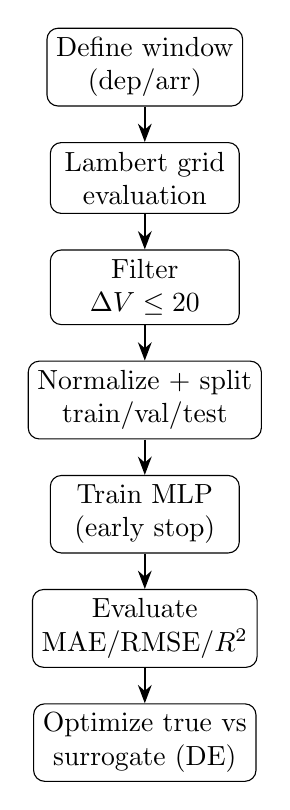
\begin{tikzpicture}[
			node distance=0.45cm,
			block/.style={
				rectangle, draw, rounded corners,
				align=center, minimum width=2.4cm, minimum height=0.65cm
			},
			arrow/.style={-{Stealth}, thick}
			]
			\node[block] (a) {Define window\\(dep/arr)};
			\node[block, below=of a] (b) {Lambert grid\\evaluation};
			\node[block, below=of b] (c) {Filter\\$\Delta V \le 20$};
			\node[block, below=of c] (d) {Normalize + split\\train/val/test};
			\node[block, below=of d] (e) {Train MLP\\(early stop)};
			\node[block, below=of e] (f) {Evaluate\\MAE/RMSE/$R^2$};
			\node[block, below=of f] (g) {Optimize true vs\\surrogate (DE)};
			\draw[arrow] (a)--(b);
			\draw[arrow] (b)--(c);
			\draw[arrow] (c)--(d);
			\draw[arrow] (d)--(e);
			\draw[arrow] (e)--(f);
			\draw[arrow] (f)--(g);
		\end{tikzpicture}
		\caption{End-to-end workflow for dataset generation, surrogate training, and optimization comparison.}
		\label{fig:flowchart}
	\end{figure}
	
	% Force all floats defined so far to appear before continuing
	\FloatBarrier
	
	% ============================================================
	\section{Results}
	\subsection{Baseline Surface and Optimization Path}
	Fig.~\ref{fig:porkchop_main} shows the Lambert pork-chop surface for the 2030--2032 window. Fig.~\ref{fig:optpath_main} overlays the DE optimization path for the true Lambert objective.
	
	\begin{figure}[!t]
		\centering
		\FIGCOL{\PLOT{\MAINRUN}{porkchop_2030-01-01_2032-01-01.png}}
		\caption{Lambert pork-chop surface for 2030--2032.}
		\label{fig:porkchop_main}
	\end{figure}
	
	\begin{figure}[!t]
		\centering
		\FIGCOL{\PLOT{\MAINRUN}{porkchop_2030-01-01_2032-01-01_optpath.png}}
		\caption{True-objective optimization path (DE) for 2030--2032.}
		\label{fig:optpath_main}
	\end{figure}
	
	\FloatBarrier
	
	\subsection{Surrogate Fidelity and Error Distributions}
	Fig.~\ref{fig:triptych_main} compares true vs surrogate and error for 2030--2032, while Fig.~\ref{fig:errhist_main} shows the error histogram.
	
	\begin{figure}[!t]
		\centering
		\FIGCOL{\PLOT{\MAINRUN}{porkchop_triptych_dep20300101-20320101_arr20300501-20321226.png}}
		\caption{Triptych for 2030--2032: true surface, surrogate prediction, and error.}
		\label{fig:triptych_main}
	\end{figure}
	
	\begin{figure}[!t]
		\centering
		\FIGCOL{\PLOT{\MAINRUN}{porkchop_error_histogram_dep20300101-20320101_arr20300501-20321226.png}}
		\caption{Error histogram for 2030--2032.}
		\label{fig:errhist_main}
	\end{figure}
	
	\FloatBarrier
	
	\subsection{Minima and Aggregate Metrics}
	Table~\ref{tab:summary} summarizes Lambert minima and surrogate errors across all windows.
	
	\begin{table}[!t]
		\caption{Summary of Minima and Surrogate Error Metrics Across Windows}
		\centering
		\resizebox{\columnwidth}{!}{%
			\begin{tabular}{lcccc}
				\toprule
				\textbf{Window} & \textbf{Grid min} & \textbf{True opt min} & \textbf{MAE} & \textbf{RMSE} \\
				& [km/s] & [km/s] & [km/s] & [km/s] \\
				\midrule
				2030--2032 & 6.7009 & 6.6445 & 0.7313 & 1.2269 \\
				2032--2034 & 6.1420 & 6.1211 & 0.7985 & 1.3743 \\
				2034--2036 & 5.5770 & 5.5707 & 1.5362 & 3.0171 \\
				2036--2038 & 6.6032 & 6.6002 & 1.5831 & 3.1374 \\
				2038--2040 & 5.7429 & 5.7125 & 1.4953 & 2.5518 \\
				\bottomrule
		\end{tabular}}
		\label{tab:summary}
	\end{table}
	
	\FloatBarrier
	
	\subsection{Four-Minima Comparison}
	Fig.~\ref{fig:fourmins_main} shows the four-minima comparison for 2030--2032.
	
	\begin{figure}[!t]
		\centering
		\FIGCOL{\PLOT{\MAINRUN}{porkchop_four_mins_dep20300101-20320101_arr20300501-20321226.png}}
		\caption{Four-minima overlay for 2030--2032.}
		\label{fig:fourmins_main}
	\end{figure}
	
	\FloatBarrier
	
	% ============================================================
	\section{Discussion}
	The surrogate reproduces dominant low-$\Delta V$ corridors for early windows and achieves sub-1~km/s MAE. Later windows show higher error and more failure cases during surrogate-based optimization, consistent with sharper gradients, fewer valid samples, and more irregular feasible regions. Because DE explores continuous bounds, the surrogate can be exploited in regions where training data are sparse; validating $J$ at surrogate optima is therefore essential. Future improvements include feasibility-aware modeling (joint feasibility classification), uncertainty-aware regression, and multi-window training.
	
	% ============================================================
	\section{Conclusion}
	This work demonstrated a supervised surrogate for approximating Earth--Mars Lambert pork-chop surfaces. Results show meaningful accuracy for early windows and highlight limitations for later windows, especially under continuous optimization. The approach supports fast trade-space exploration for preliminary mission design while motivating feasibility-aware extensions.
	
	% ============================================================
	\begin{thebibliography}{00}
		\bibitem{zavoli2021}
		A.~Zavoli and L.~Federici, ``Reinforcement learning for robust trajectory design of interplanetary missions,'' \emph{Journal of Guidance, Control, and Dynamics}, vol.~44, no.~8, pp.~1447--1459, 2021.
		
		\bibitem{ruff2023}
		E.~Ruff, R.~Russell, M.~Stoeckle, P.~Miotto, and J.~P.~How, ``Surrogate neural networks for efficient simulation-based trajectory planning optimization,'' arXiv preprint arXiv:2303.17468, 2023.
		
		\bibitem{federici2024}
		L.~Federici and A.~Zavoli, ``Robust interplanetary trajectory design under multiple uncertainties via meta-reinforcement learning,'' \emph{Acta Astronautica}, 2024.
	\end{thebibliography}
	
	% ============================================================
	% BACKUP FIGURES: start on a new page, single-column, full width
	% Use [H] so they DO NOT MOVE in the appendix.
	% ============================================================
	\clearpage
	\onecolumn
	\appendix
	\section*{Appendix: Additional Windows (Backup Figures)}
	
	\subsection*{2032--2034}
	\begin{figure}[H]
		\centering
		\FIGFULL{\PLOT{dep2032-01-01_2034-01-01_arr2032-05-01_2034-12-26}{porkchop_2032-01-01_2034-01-01.png}}
		\caption{Lambert pork-chop surface for 2032--2034.}
	\end{figure}
	
	\begin{figure}[H]
		\centering
		\FIGFULL{\PLOT{dep2032-01-01_2034-01-01_arr2032-05-01_2034-12-26}{porkchop_2032-01-01_2034-01-01_optpath.png}}
		\caption{True-objective optimization path for 2032--2034.}
	\end{figure}
	
	\begin{figure}[H]
		\centering
		\FIGFULL{\PLOT{dep2032-01-01_2034-01-01_arr2032-05-01_2034-12-26}{porkchop_triptych_dep20320101-20340101_arr20320430-20341227.png}}
		\caption{Triptych for 2032--2034: true surface, surrogate prediction, and error.}
	\end{figure}
	
	\begin{figure}[H]
		\centering
		\FIGFULL{\PLOT{dep2032-01-01_2034-01-01_arr2032-05-01_2034-12-26}{porkchop_error_histogram_dep20320101-20340101_arr20320430-20341227.png}}
		\caption{Error histogram for 2032--2034.}
	\end{figure}
	
	\begin{figure}[H]
		\centering
		\FIGFULL{\PLOT{dep2032-01-01_2034-01-01_arr2032-05-01_2034-12-26}{porkchop_four_mins_dep20320101-20340101_arr20320430-20341227.png}}
		\caption{Four-minima overlay for 2032--2034.}
	\end{figure}
	
	\clearpage
	\subsection*{2034--2036}
	\begin{figure}[H]
		\centering
		\FIGFULL{\PLOT{dep2034-01-01_2036-01-01_arr2034-05-01_2036-12-26}{porkchop_2034-01-01_2036-01-01.png}}
		\caption{Lambert pork-chop surface for 2034--2036.}
	\end{figure}
	
	\begin{figure}[H]
		\centering
		\FIGFULL{\PLOT{dep2034-01-01_2036-01-01_arr2034-05-01_2036-12-26}{porkchop_2034-01-01_2036-01-01_optpath.png}}
		\caption{True-objective optimization path for 2034--2036.}
	\end{figure}
	
	\begin{figure}[H]
		\centering
		\FIGFULL{\PLOT{dep2034-01-01_2036-01-01_arr2034-05-01_2036-12-26}{porkchop_triptych_dep20340101-20360101_arr20340501-20361226.png}}
		\caption{Triptych for 2034--2036: true surface, surrogate prediction, and error.}
	\end{figure}
	
	\begin{figure}[H]
		\centering
		\FIGFULL{\PLOT{dep2034-01-01_2036-01-01_arr2034-05-01_2036-12-26}{porkchop_error_histogram_dep20340101-20360101_arr20340501-20361226.png}}
		\caption{Error histogram for 2034--2036.}
	\end{figure}
	
	\begin{figure}[H]
		\centering
		\FIGFULL{\PLOT{dep2034-01-01_2036-01-01_arr2034-05-01_2036-12-26}{porkchop_four_mins_dep20340101-20360101_arr20340501-20361226.png}}
		\caption{Four-minima overlay for 2034--2036.}
	\end{figure}
	
	\clearpage
	\subsection*{2036--2038}
	\begin{figure}[H]
		\centering
		\FIGFULL{\PLOT{dep2036-01-01_2038-01-01_arr2036-05-01_2038-12-26}{porkchop_2036-01-01_2038-01-01.png}}
		\caption{Lambert pork-chop surface for 2036--2038.}
	\end{figure}
	
	\begin{figure}[H]
		\centering
		\FIGFULL{\PLOT{dep2036-01-01_2038-01-01_arr2036-05-01_2038-12-26}{porkchop_2036-01-01_2038-01-01_optpath.png}}
		\caption{True-objective optimization path for 2036--2038.}
	\end{figure}
	
	\begin{figure}[H]
		\centering
		\FIGFULL{\PLOT{dep2036-01-01_2038-01-01_arr2036-05-01_2038-12-26}{porkchop_triptych_dep20360101-20380101_arr20360430-20381227.png}}
		\caption{Triptych for 2036--2038: true surface, surrogate prediction, and error.}
	\end{figure}
	
	\begin{figure}[H]
		\centering
		\FIGFULL{\PLOT{dep2036-01-01_2038-01-01_arr2036-05-01_2038-12-26}{porkchop_error_histogram_dep20360101-20380101_arr20360430-20381227.png}}
		\caption{Error histogram for 2036--2038.}
	\end{figure}
	
	\begin{figure}[H]
		\centering
		\FIGFULL{\PLOT{dep2036-01-01_2038-01-01_arr2036-05-01_2038-12-26}{porkchop_four_mins_dep20360101-20380101_arr20360430-20381227.png}}
		\caption{Four-minima overlay for 2036--2038.}
	\end{figure}
	
	\clearpage
	\subsection*{2038--2040}
	\begin{figure}[H]
		\centering
		\FIGFULL{\PLOT{dep2038-01-01_2040-01-01_arr2038-05-01_2040-12-26}{porkchop_2038-01-01_2040-01-01.png}}
		\caption{Lambert pork-chop surface for 2038--2040.}
	\end{figure}
	
	\begin{figure}[H]
		\centering
		\FIGFULL{\PLOT{dep2038-01-01_2040-01-01_arr2038-05-01_2040-12-26}{porkchop_2038-01-01_2040-01-01_optpath.png}}
		\caption{True-objective optimization path for 2038--2040.}
	\end{figure}
	
	\begin{figure}[H]
		\centering
		\FIGFULL{\PLOT{dep2038-01-01_2040-01-01_arr2038-05-01_2040-12-26}{porkchop_triptych_dep20380101-20400101_arr20380501-20401226.png}}
		\caption{Triptych for 2038--2040: true surface, surrogate prediction, and error.}
	\end{figure}
	
	\begin{figure}[H]
		\centering
		\FIGFULL{\PLOT{dep2038-01-01_2040-01-01_arr2038-05-01_2040-12-26}{porkchop_error_histogram_dep20380101-20400101_arr20380501-20401226.png}}
		\caption{Error histogram for 2038--2040.}
	\end{figure}
	
	\begin{figure}[H]
		\centering
		\FIGFULL{\PLOT{dep2038-01-01_2040-01-01_arr2038-05-01_2040-12-26}{porkchop_four_mins_dep20380101-20400101_arr20380501-20401226.png}}
		\caption{Four-minima overlay for 2038--2040.}
	\end{figure}
	
	\appendix
	\section{Code}
	
	\begin{lstlisting}[language=Python, caption={Main Code}]
		import os
		import sys
		import atexit
		from datetime import datetime
		import pandas as pd
		from tqdm import tqdm
		
		from porkchop_run import (
		generate_porkchop_data_daily,
		plot_porkchop,
		find_global_min_from_grid,
		run_optimizer_with_history,
		plot_porkchop_with_trajectory,
		prepare_ml_npz_from_csv,
		)
		
		from train_surrogate import train_from_npz
		from evaluate_surrogate import evaluate_surrogate
		
		
		class Tee:
		def __init__(self, *streams):
		self.streams = streams
		
		def write(self, data):
		for s in self.streams:
		try:
		s.write(data)
		s.flush()
		except Exception:
		pass
		
		def flush(self):
		for s in self.streams:
		try:
		s.flush()
		except Exception:
		pass
		
		
		def ensure_dir(path):
		os.makedirs(path, exist_ok=True)
		
		
		def combo_tag(dep_start, dep_end, arr_start, arr_end):
		return f"dep{dep_start}_{dep_end}_arr{arr_start}_{arr_end}"
		
		
		run_tag = datetime.now().strftime("%Y%m%d_%H%M%S")
		base_out_dir = os.path.abspath(f"runs_{run_tag}")
		ensure_dir(base_out_dir)
		
		log_name = os.path.abspath(f"run_log_{run_tag}.txt")
		log_file = open(log_name, "w", encoding="utf-8")
		
		sys.stdout = Tee(sys.__stdout__, log_file)
		sys.stderr = Tee(sys.__stderr__, log_file)
		
		print(f"Logging console output to: {log_name}")
		
		
		def _close_log():
		try:
		log_file.flush()
		log_file.close()
		except Exception:
		pass
		
		
		atexit.register(_close_log)
		
		
		min_tof = 120.0
		max_tof = 360.0
		n_tof = 60
		dv_cutoff = 20.0
		
		years = [2030, 2032, 2034, 2036, 2038]
		
		for y0 in tqdm(years, desc="Running porkchop + surrogate experiments", unit="window", ncols=100):
		dep_start = f"{y0}-01-01"
		dep_end = f"{y0 + 2}-01-01"
		arr_start = f"{y0}-05-01"
		arr_end = f"{y0 + 2}-12-26"
		
		tag = combo_tag(dep_start, dep_end, arr_start, arr_end)
		out_dir = os.path.abspath(os.path.join(base_out_dir, tag))
		ensure_dir(out_dir)
		
		print("\n" + "=" * 80)
		print(f"RUN COMBO: {tag}")
		print("=" * 80)
		
		csv_name = f"porkchop_{tag}.csv"
		clean_csv_name = f"porkchop_{tag}_clean.csv"
		npz_name = f"ml_data_{tag}.npz"
		norm_name = f"normalization_stats_{tag}.json"
		model_name = f"dv_surrogate_model_{tag}.pt"
		
		csv_path = os.path.join(out_dir, csv_name)
		clean_csv_path = os.path.join(out_dir, clean_csv_name)
		npz_path = os.path.join(out_dir, npz_name)
		norm_path = os.path.join(out_dir, norm_name)
		model_path = os.path.join(out_dir, model_name)
		
		df, dep_times, tofs_days, dv_grid = generate_porkchop_data_daily(
		dep_start=dep_start,
		dep_end=dep_end,
		arr_start=arr_start,
		arr_end=arr_end,
		min_tof_days=min_tof,
		max_tof_days=max_tof,
		n_tof=n_tof,
		csv_path=csv_path,
		dv_cutoff=dv_cutoff,
		n_jobs=-1,
		)
		
		old_cwd = os.getcwd()
		os.chdir(out_dir)
		try:
		plot_porkchop(dep_times, tofs_days, dv_grid, title_suffix=f"{dep_start}_{dep_end}")
		finally:
		os.chdir(old_cwd)
		
		global_min = find_global_min_from_grid(dep_times, tofs_days, dv_grid)
		print("GRID MIN")
		print(global_min["dep_time"].iso)
		print(f"{global_min['tof_days']:.6f}")
		print(global_min["arr_time"].iso)
		print(f"{global_min['dv_kms']:.6f}")
		
		opt_result = run_optimizer_with_history(
		dep_start=dep_start,
		dep_end=dep_end,
		min_tof_days=min_tof,
		max_tof_days=max_tof,
		dv_cutoff=dv_cutoff,
		method="de",
		seed=1,
		)
		
		print("OPT MIN")
		print(opt_result["dep_time"].iso)
		print(f"{opt_result['tof_days']:.6f}")
		print(opt_result["arr_time"].iso)
		print(f"{opt_result['dv_kms']:.6f}")
		print(len(opt_result["history"]))
		
		os.chdir(out_dir)
		try:
		plot_porkchop_with_trajectory(
		dep_times,
		tofs_days,
		dv_grid,
		global_min=global_min,
		opt_result=opt_result,
		title_suffix=f"{dep_start}_{dep_end}",
		)
		finally:
		os.chdir(old_cwd)
		
		if not os.path.exists(clean_csv_path):
		df_raw = pd.read_csv(csv_path)
		df_clean = df_raw.dropna(subset=["dv_total_kms"]).copy()
		df_clean.to_csv(clean_csv_path, index=False)
		print(f"Saved clean CSV: {clean_csv_path}")
		else:
		print(f"Clean CSV exists: {clean_csv_path}")
		
		prepare_ml_npz_from_csv(csv_path, out_npz=npz_path, out_norm_json=norm_path)
		train_from_npz(npz_path, save_path=model_path)
		
		os.chdir(out_dir)
		try:
		evaluate_surrogate(
		dep_start=dep_start,
		dep_end=dep_end,
		min_tof_days=min_tof,
		max_tof_days=max_tof,
		clean_csv_path=clean_csv_name,
		model_checkpoint=model_name,
		norm_stats_path=norm_name,
		true_opt_result=opt_result,
		dv_cutoff=dv_cutoff,
		surrogate_opt_method="de",
		surrogate_opt_seed=2,
		)
		finally:
		os.chdir(old_cwd)
		
		print("\nALL COMBINATIONS COMPLETE")
		print(f"Results saved under: {base_out_dir}")
		
	\end{lstlisting}
	
	\newpage
	
	\begin{lstlisting}[language=Python, caption={Data Generation}]
		#!/usr/bin/env python
		# -*- coding: utf-8 -*-
		
		import os
		import json
		import argparse
		import numpy as np
		import pandas as pd
		
		from astropy import units as u
		from astropy.time import Time, TimeDelta
		
		import matplotlib.pyplot as plt
		import matplotlib.dates as mdates
		
		from poliastro.bodies import Sun, Earth, Mars
		from poliastro.twobody import Orbit
		from poliastro.iod import izzo
		
		from tqdm.auto import tqdm
		
		try:
		from joblib import Parallel, delayed
		_HAS_JOBLIB = True
		except Exception:
		_HAS_JOBLIB = False
		
		try:
		from poliastro.ephem import Ephem
		_HAS_EPHEM = True
		except Exception:
		_HAS_EPHEM = False
		
		try:
		from scipy.optimize import differential_evolution, minimize
		_HAS_SCIPY = True
		except Exception:
		_HAS_SCIPY = False
		
		DV_CUTOFF = 20.0
		DATA_CSV_PATH = "porkchop_earth_mars_2030_2032_daily.csv"
		N_JOBS = -1
		
		
		def get_heliocentric_state(body, epoch):
		orb = Orbit.from_body_ephem(body, epoch)
		return orb.r, orb.v
		
		
		def lambert_delta_v(r1, v1_planet, r2, v2_planet, tof_seconds):
		(v1_trans, v2_trans), = izzo.lambert(Sun.k, r1, r2, tof_seconds)
		dv1_vec = v1_trans - v1_planet
		dv2_vec = v2_planet - v2_trans
		dv1 = np.linalg.norm(dv1_vec.to(u.km / u.s).value)
		dv2 = np.linalg.norm(dv2_vec.to(u.km / u.s).value)
		return dv1 + dv2, dv1, dv2
		
		
		def delta_v_objective(dep_time, tof_days, dv_cutoff=DV_CUTOFF, return_components=False):
		try:
		tof_days = float(tof_days)
		if tof_days <= 0.0:
		return (np.nan, np.nan, np.nan) if return_components else np.nan
		
		tof_seconds = (tof_days * u.day).to(u.s)
		r_E, v_E = get_heliocentric_state(Earth, dep_time)
		arr_time = dep_time + TimeDelta(tof_days * u.day)
		r_M, v_M = get_heliocentric_state(Mars, arr_time)
		dv_total, dv1, dv2 = lambert_delta_v(r_E, v_E, r_M, v_M, tof_seconds)
		
		if (not np.isfinite(dv_total)) or (dv_total > dv_cutoff):
		return (np.nan, np.nan, np.nan) if return_components else np.nan
		
		return (dv_total, dv1, dv2) if return_components else dv_total
		
		except Exception:
		return (np.nan, np.nan, np.nan) if return_components else np.nan
		
		
		def _mars_states_vectorized(arr_times):
		if _HAS_EPHEM:
		try:
		eph = Ephem.from_body(Mars, arr_times)
		r_M, v_M = eph.rv(arr_times)
		r_list = [r_M[i] for i in range(len(arr_times))]
		v_list = [v_M[i] for i in range(len(arr_times))]
		return r_list, v_list
		except Exception:
		pass
		
		r_list, v_list = [], []
		for t in arr_times:
		r, v = get_heliocentric_state(Mars, t)
		r_list.append(r)
		v_list.append(v)
		return r_list, v_list
		
		
		def _compute_one_departure_fast(t_dep, tofs_days, dv_cutoff):
		n_tof = len(tofs_days)
		
		dv_row = np.full(n_tof, np.nan, dtype=np.float64)
		dv1_row = np.full(n_tof, np.nan, dtype=np.float64)
		dv2_row = np.full(n_tof, np.nan, dtype=np.float64)
		
		r_E, v_E = get_heliocentric_state(Earth, t_dep)
		
		arr_times = t_dep + TimeDelta(tofs_days * u.day)
		arr_tdb = arr_times.tdb
		
		arr_jd_row = arr_tdb.jd.astype(np.float64)
		arr_iso_row = arr_tdb.iso.astype(object)
		
		r_M_list, v_M_list = _mars_states_vectorized(arr_times)
		
		for j, tof_days in enumerate(tofs_days):
		try:
		tof_seconds = (float(tof_days) * u.day).to(u.s)
		dv_total, dv1, dv2 = lambert_delta_v(r_E, v_E, r_M_list[j], v_M_list[j], tof_seconds)
		
		if (not np.isfinite(dv_total)) or (dv_total > dv_cutoff):
		continue
		
		dv_row[j] = dv_total
		dv1_row[j] = dv1
		dv2_row[j] = dv2
		except Exception:
		continue
		
		return dv_row, dv1_row, dv2_row, arr_jd_row, arr_iso_row
		
		
		def generate_porkchop_data_daily(
		dep_start="2030-01-01",
		dep_end="2032-01-01",
		arr_start=None,
		arr_end=None,
		departure_step_days=1,
		min_tof_days=100.0,
		max_tof_days=400.0,
		n_tof=60,
		csv_path=DATA_CSV_PATH,
		dv_cutoff=DV_CUTOFF,
		n_jobs=N_JOBS,
		):
		t_dep_start = Time(dep_start, scale="tdb").tdb
		t_dep_end = Time(dep_end, scale="tdb").tdb
		
		if arr_start is not None and arr_end is not None:
		t_arr_start = Time(arr_start, scale="tdb").tdb
		t_arr_end = Time(arr_end, scale="tdb").tdb
		min_tof = (t_arr_start - t_dep_end).to(u.day).value
		max_tof = (t_arr_end - t_dep_start).to(u.day).value
		min_tof_days = float(max(min_tof, 1.0))
		max_tof_days = float(max(max_tof, min_tof_days + 1.0))
		print(f"Derived TOF range: [{min_tof_days:.3f}, {max_tof_days:.3f}] days")
		
		total_days = int((t_dep_end - t_dep_start).to(u.day).value)
		day_offsets = np.arange(0, total_days + 1, int(departure_step_days), dtype=int)
		dep_times = (t_dep_start + TimeDelta(day_offsets * u.day)).tdb
		n_departures = len(dep_times)
		
		tofs_days = np.linspace(float(min_tof_days), float(max_tof_days), int(n_tof), dtype=np.float64)
		n_tof = len(tofs_days)
		
		print(f"Grid: {n_departures} departures × {n_tof} TOFs")
		print(f"Departure window: {t_dep_start.iso} to {t_dep_end.iso}")
		if arr_start is not None and arr_end is not None:
		print(f"Arrival window: {Time(arr_start, scale='tdb').tdb.iso} to {Time(arr_end, scale='tdb').tdb.iso}")
		print(f"DV cutoff: {dv_cutoff} km/s")
		if not _HAS_EPHEM:
		print("Ephem unavailable; Mars ephemeris will be slower.")
		
		dep_jd = dep_times.jd.astype(np.float64)
		dep_iso = dep_times.iso.astype(object)
		
		dv_grid = np.full((n_departures, n_tof), np.nan, dtype=np.float64)
		dv1_grid = np.full((n_departures, n_tof), np.nan, dtype=np.float64)
		dv2_grid = np.full((n_departures, n_tof), np.nan, dtype=np.float64)
		
		arr_jd_grid = np.empty((n_departures, n_tof), dtype=np.float64)
		arr_iso_grid = np.empty((n_departures, n_tof), dtype=object)
		
		do_parallel = _HAS_JOBLIB and isinstance(n_jobs, int) and (n_jobs != 1) and (n_departures > 1)
		
		if do_parallel:
		results = Parallel(n_jobs=n_jobs, prefer="processes")(
		delayed(_compute_one_departure_fast)(dep_times[i], tofs_days, dv_cutoff)
		for i in range(n_departures)
		)
		for i, (dv_row, dv1_row, dv2_row, arr_jd_row, arr_iso_row) in enumerate(results):
		dv_grid[i, :] = dv_row
		dv1_grid[i, :] = dv1_row
		dv2_grid[i, :] = dv2_row
		arr_jd_grid[i, :] = arr_jd_row
		arr_iso_grid[i, :] = arr_iso_row
		else:
		for i, t_dep in enumerate(tqdm(dep_times, desc="Departures", unit="dep")):
		dv_row, dv1_row, dv2_row, arr_jd_row, arr_iso_row = _compute_one_departure_fast(
		t_dep, tofs_days, dv_cutoff
		)
		dv_grid[i, :] = dv_row
		dv1_grid[i, :] = dv1_row
		dv2_grid[i, :] = dv2_row
		arr_jd_grid[i, :] = arr_jd_row
		arr_iso_grid[i, :] = arr_iso_row
		
		n_total = n_departures * n_tof
		dep_jd_flat = np.repeat(dep_jd, n_tof)
		dep_iso_flat = np.repeat(dep_iso, n_tof)
		tof_flat = np.tile(tofs_days, n_departures)
		
		df = pd.DataFrame(
		{
			"dep_julian": dep_jd_flat,
			"arr_julian": arr_jd_grid.reshape(n_total),
			"dep_iso": dep_iso_flat,
			"arr_iso": arr_iso_grid.reshape(n_total),
			"tof_days": tof_flat.astype(np.float64),
			"dv_total_kms": dv_grid.reshape(n_total),
			"dv_dep_kms": dv1_grid.reshape(n_total),
			"dv_arr_kms": dv2_grid.reshape(n_total),
		}
		)
		
		if arr_start is not None and arr_end is not None:
		t_arr_start = Time(arr_start, scale="tdb").tdb
		t_arr_end = Time(arr_end, scale="tdb").tdb
		arr_t = Time(df["arr_julian"].values.astype(np.float64), format="jd", scale="tdb").tdb
		in_window = (arr_t.jd >= t_arr_start.jd) & (arr_t.jd <= t_arr_end.jd)
		df.loc[~in_window, ["dv_total_kms", "dv_dep_kms", "dv_arr_kms"]] = np.nan
		
		df.to_csv(csv_path, index=False)
		print(f"Saved CSV: {csv_path} ({len(df)} rows)")
		return df, dep_times, tofs_days, dv_grid
		
		
		def plot_porkchop(dep_times, tofs_days, dv_grid, title_suffix="run"):
		os.makedirs("plots", exist_ok=True)
		
		dep_datetimes = dep_times.to_datetime()
		dep_mpl = mdates.date2num(dep_datetimes)
		
		D_dep, D_tof = np.meshgrid(dep_mpl, tofs_days, indexing="ij")
		Z = np.ma.masked_invalid(dv_grid)
		
		plt.figure(figsize=(10, 5))
		cs = plt.contourf(D_dep, D_tof, Z, levels=30)
		cbar = plt.colorbar(cs)
		cbar.set_label(r"Total $\Delta V$ [km/s]")
		
		try:
		cs_lines = plt.contour(D_dep, D_tof, Z, levels=10, colors="k", linewidths=0.5)
		plt.clabel(cs_lines, inline=True, fontsize=8, fmt="%.1f")
		except Exception:
		pass
		
		ax = plt.gca()
		ax.xaxis.set_major_formatter(mdates.DateFormatter("%Y-%m-%d"))
		ax.xaxis.set_major_locator(mdates.AutoDateLocator())
		
		plt.xticks(rotation=30, ha="right")
		plt.xlabel("Departure Date")
		plt.ylabel("Time of Flight [days]")
		plt.title(rf"Earth–Mars Pork-Chop (Total $\Delta V$) {title_suffix}")
		
		plt.tight_layout()
		save_path = f"plots/porkchop_{title_suffix}.png"
		plt.savefig(save_path, dpi=300)
		print(f"Saved plot: {save_path}")
		
		def rebuild_grid_from_csv(df):
		dep_julians = np.sort(df["dep_julian"].unique())
		tofs_days = np.sort(df["tof_days"].unique())
		dep_times = Time(dep_julians, format="jd", scale="tdb").tdb
		
		grid = (
		df.pivot(index="dep_julian", columns="tof_days", values="dv_total_kms")
		.reindex(index=dep_julians, columns=tofs_days)
		.to_numpy()
		)
		return dep_times, tofs_days, grid
		
		
		def find_global_min_from_grid(dep_times, tofs_days, dv_grid):
		Z = np.array(dv_grid, dtype=np.float64)
		if not np.isfinite(Z).any():
		raise RuntimeError("dv_grid has no finite values")
		idx = np.nanargmin(Z)
		i, j = np.unravel_index(idx, Z.shape)
		dep_time = dep_times[i].tdb
		tof = float(tofs_days[j])
		arr_time = (dep_time + TimeDelta(tof * u.day)).tdb
		dv = float(Z[i, j])
		return {"i": int(i), "j": int(j), "dep_time": dep_time, "tof_days": tof, "arr_time": arr_time, "dv_kms": dv}
		
		
		def _continuous_objective_factory(dv_cutoff, dep_jd_bounds, tof_bounds):
		dep_lo, dep_hi = dep_jd_bounds
		tof_lo, tof_hi = tof_bounds
		BIG = 1e6
		
		def f(x):
		dep_jd = float(x[0])
		tof_days = float(x[1])
		
		if dep_jd < dep_lo or dep_jd > dep_hi or tof_days < tof_lo or tof_days > tof_hi:
		return BIG
		
		dep_time = Time(dep_jd, format="jd", scale="tdb").tdb
		dv = delta_v_objective(dep_time, tof_days, dv_cutoff=dv_cutoff, return_components=False)
		if (dv is None) or (not np.isfinite(dv)):
		return BIG
		return float(dv)
		
		return f
		
		
		def run_optimizer_with_history(
		dep_start, dep_end,
		min_tof_days, max_tof_days,
		dv_cutoff=DV_CUTOFF,
		method="de",
		seed=1,
		):
		if not _HAS_SCIPY:
		raise RuntimeError("SciPy not available")
		
		t0 = Time(dep_start, scale="tdb").tdb
		t1 = Time(dep_end, scale="tdb").tdb
		
		dep_bounds = (float(t0.jd), float(t1.jd))
		tof_bounds = (float(min_tof_days), float(max_tof_days))
		
		f = _continuous_objective_factory(dv_cutoff, dep_bounds, tof_bounds)
		history = []
		
		x0 = np.array([(dep_bounds[0] + dep_bounds[1]) / 2.0, (tof_bounds[0] + tof_bounds[1]) / 2.0], dtype=float)
		
		if method.lower() == "de":
		bounds = [dep_bounds, tof_bounds]
		
		def cb(xk, convergence=None):
		history.append((float(xk[0]), float(xk[1]), float(f(xk))))
		return False
		
		res = differential_evolution(
		f,
		bounds=bounds,
		seed=seed,
		callback=cb,
		polish=True,
		updating="deferred",
		workers=1,
		)
		xbest = res.x
		else:
		bounds = [dep_bounds, tof_bounds]
		
		def cb(xk):
		history.append((float(xk[0]), float(xk[1]), float(f(xk))))
		
		res = minimize(
		f,
		x0=x0,
		method="L-BFGS-B",
		bounds=bounds,
		callback=cb,
		)
		xbest = res.x
		
		dep_jd_best = float(xbest[0])
		tof_best = float(xbest[1])
		dep_time_best = Time(dep_jd_best, format="jd", scale="tdb").tdb
		arr_time_best = (dep_time_best + TimeDelta(tof_best * u.day)).tdb
		dv_best = float(delta_v_objective(dep_time_best, tof_best, dv_cutoff=dv_cutoff))
		
		return {
			"method": method,
			"success": bool(getattr(res, "success", True)),
			"message": str(getattr(res, "message", "")),
			"nfev": int(getattr(res, "nfev", -1)) if getattr(res, "nfev", None) is not None else -1,
			"dep_time": dep_time_best,
			"tof_days": tof_best,
			"arr_time": arr_time_best,
			"dv_kms": dv_best,
			"history": history,
		}
		
		
		def plot_porkchop_with_trajectory(dep_times, tofs_days, dv_grid, global_min, opt_result, title_suffix="opt"):
		os.makedirs("plots", exist_ok=True)
		
		dep_datetimes = dep_times.to_datetime()
		dep_mpl = mdates.date2num(dep_datetimes)
		
		D_dep, D_tof = np.meshgrid(dep_mpl, tofs_days, indexing="ij")
		Z = np.ma.masked_invalid(dv_grid)
		
		plt.figure(figsize=(10, 5))
		cs = plt.contourf(D_dep, D_tof, Z, levels=30)
		cbar = plt.colorbar(cs)
		cbar.set_label(r"Total $\Delta V$ [km/s]")
		
		ax = plt.gca()
		ax.xaxis.set_major_formatter(mdates.DateFormatter("%Y-%m-%d"))
		ax.xaxis.set_major_locator(mdates.AutoDateLocator())
		plt.xticks(rotation=30, ha="right")
		plt.xlabel("Departure Date")
		plt.ylabel("Time of Flight [days]")
		
		g_dep = mdates.date2num(global_min["dep_time"].to_datetime())
		g_tof = float(global_min["tof_days"])
		plt.scatter([g_dep], [g_tof], marker="*", s=180, label=f"Grid min: {global_min['dv_kms']:.3f} km/s")
		
		hist = opt_result.get("history", [])
		if len(hist) > 0:
		hist_dep_dt = [Time(h[0], format="jd", scale="tdb").to_datetime() for h in hist]
		hist_dep_mpl = mdates.date2num(hist_dep_dt)
		hist_tof = [h[1] for h in hist]
		plt.plot(hist_dep_mpl, hist_tof, linewidth=2, label=f"Opt path ({opt_result['method']})")
		plt.scatter([hist_dep_mpl[-1]], [hist_tof[-1]], marker="o", s=60)
		
		o_dep = mdates.date2num(opt_result["dep_time"].to_datetime())
		o_tof = float(opt_result["tof_days"])
		plt.scatter([o_dep], [o_tof], marker="X", s=120, label=f"Opt min: {opt_result['dv_kms']:.3f} km/s")
		
		plt.title(rf"Pork-Chop + Opt Path ({title_suffix})")
		plt.legend(loc="best")
		plt.tight_layout()
		
		save_path = f"plots/porkchop_{title_suffix}_optpath.png"
		plt.savefig(save_path, dpi=300)
		print(f"Saved plot: {save_path}")
		
		def prepare_ml_npz_from_csv(csv_path, out_npz="ml_data_all.npz", out_norm_json="normalization_stats.json"):
		df = pd.read_csv(csv_path)
		df_clean = df.dropna(subset=["dv_total_kms"]).copy()
		
		X = df_clean[["dep_julian", "tof_days"]].values.astype(np.float32)
		y = df_clean["dv_total_kms"].values.astype(np.float32).reshape(-1, 1)
		
		dep_julian = df_clean["dep_julian"].values.astype(np.float64)
		dep_year = df_clean["dep_iso"].str.slice(0, 4).astype(np.int16).values
		
		X_mean = X.mean(axis=0)
		X_std = X.std(axis=0)
		X_std[X_std == 0.0] = 1.0
		X_norm = (X - X_mean) / X_std
		
		with open(out_norm_json, "w") as f:
		json.dump({"X_mean": X_mean.tolist(), "X_std": X_std.tolist()}, f)
		
		np.savez(
		out_npz,
		X_norm=X_norm,
		y=y,
		dep_julian=dep_julian,
		dep_year=dep_year,
		)
		
		print(f"Saved: {out_norm_json}")
		print(f"Saved: {out_npz}")
		print(f"Rows: {len(df_clean)} / {len(df)}")
		return out_npz
		
		
		def parse_args():
		p = argparse.ArgumentParser(description="Earth->Mars porkchop generator")
		
		p.add_argument("--dep-start", type=str, default="2030-01-01")
		p.add_argument("--dep-end", type=str, default="2032-01-01")
		p.add_argument("--arr-start", type=str, default=None)
		p.add_argument("--arr-end", type=str, default=None)
		
		p.add_argument("--dep-step", type=int, default=1)
		p.add_argument("--min-tof", type=float, default=120.0)
		p.add_argument("--max-tof", type=float, default=360.0)
		p.add_argument("--n-tof", type=int, default=60)
		
		p.add_argument("--dv-cutoff", type=float, default=DV_CUTOFF)
		p.add_argument("--csv", type=str, default=DATA_CSV_PATH)
		p.add_argument("--n-jobs", type=int, default=N_JOBS)
		
		p.add_argument("--no-generate", action="store_true")
		p.add_argument("--plot", action="store_true")
		p.add_argument("--opt-plot", action="store_true")
		p.add_argument("--opt-method", type=str, default="de", choices=["de", "lbfgsb"])
		p.add_argument("--opt-seed", type=int, default=1)
		p.add_argument("--prep-ml", action="store_true")
		p.add_argument("--title", type=str, default="run")
		
		return p.parse_args()
		
		
		if __name__ == "__main__":
		args = parse_args()
		
		dep_times = None
		tofs_days = None
		dv_grid = None
		
		if not args.no_generate:
		_, dep_times, tofs_days, dv_grid = generate_porkchop_data_daily(
		dep_start=args.dep_start,
		dep_end=args.dep_end,
		arr_start=args.arr_start,
		arr_end=args.arr_end,
		departure_step_days=args.dep_step,
		min_tof_days=args.min_tof,
		max_tof_days=args.max_tof,
		n_tof=args.n_tof,
		csv_path=args.csv,
		dv_cutoff=args.dv_cutoff,
		n_jobs=args.n_jobs,
		)
		
		if args.plot:
		if dep_times is None or tofs_days is None or dv_grid is None:
		df_plot = pd.read_csv(args.csv)
		dep_times, tofs_days, dv_grid = rebuild_grid_from_csv(df_plot)
		plot_porkchop(dep_times, tofs_days, dv_grid, title_suffix=args.title)
		
		if args.opt_plot:
		if dep_times is None or tofs_days is None or dv_grid is None:
		df_plot = pd.read_csv(args.csv)
		dep_times, tofs_days, dv_grid = rebuild_grid_from_csv(df_plot)
		
		global_min = find_global_min_from_grid(dep_times, tofs_days, dv_grid)
		print(f"Grid min dep: {global_min['dep_time'].iso}")
		print(f"Grid min tof: {global_min['tof_days']:.6f}")
		print(f"Grid min arr: {global_min['arr_time'].iso}")
		print(f"Grid min dv:  {global_min['dv_kms']:.6f}")
		
		opt_result = run_optimizer_with_history(
		dep_start=args.dep_start,
		dep_end=args.dep_end,
		min_tof_days=args.min_tof,
		max_tof_days=args.max_tof,
		dv_cutoff=args.dv_cutoff,
		method=args.opt_method,
		seed=args.opt_seed,
		)
		
		print(f"Opt min dep:  {opt_result['dep_time'].iso}")
		print(f"Opt min tof:  {opt_result['tof_days']:.6f}")
		print(f"Opt min arr:  {opt_result['arr_time'].iso}")
		print(f"Opt min dv:   {opt_result['dv_kms']:.6f}")
		print(f"History pts:  {len(opt_result['history'])}")
		
		plot_porkchop_with_trajectory(
		dep_times, tofs_days, dv_grid,
		global_min=global_min,
		opt_result=opt_result,
		title_suffix=args.title,
		)
		
		if args.prep_ml:
		prepare_ml_npz_from_csv(args.csv, out_npz="ml_data_all.npz", out_norm_json="normalization_stats.json")
		
	\end{lstlisting}
	
	\newpage
	
	\begin{lstlisting}[language=Python, caption={Train Data}]
		import json
		import random
		import numpy as np
		import torch
		import torch.nn as nn
		import torch.optim as optim
		from torch.utils.data import TensorDataset, DataLoader
		
		DATA_NPZ_PATH = "ml_data_all.npz"
		
		N_EPOCHS = 200
		BATCH_SIZE = 128
		LR = 3e-4
		PATIENCE = 20
		
		DEVICE = "cuda" if torch.cuda.is_available() else "cpu"
		
		
		def load_ml_data(npz_path=DATA_NPZ_PATH):
		data = np.load(npz_path)
		X_norm = data["X_norm"]
		y = data["y"]
		dep_j = data["dep_julian"]
		dep_year = data["dep_year"]
		
		idx = np.argsort(dep_j)
		X_norm = X_norm[idx]
		y = y[idx]
		dep_j = dep_j[idx]
		dep_year = dep_year[idx]
		
		return X_norm, y, dep_j, dep_year
		
		
		def train_val_test_split(X, y, dep_j, train_frac=0.7, val_frac=0.15):
		N = len(dep_j)
		n_train = int(train_frac * N)
		n_val = int(val_frac * N)
		
		X_train = X[:n_train]
		y_train = y[:n_train]
		
		X_val = X[n_train:n_train + n_val]
		y_val = y[n_train:n_train + n_val]
		
		X_test = X[n_train + n_val:]
		y_test = y[n_train + n_val:]
		
		dep_train = dep_j[:n_train]
		dep_val = dep_j[n_train:n_train + n_val]
		dep_test = dep_j[n_train + n_val:]
		
		print("Split sizes:")
		print(f"  Train: {X_train.shape[0]}")
		print(f"  Val:   {X_val.shape[0]}")
		print(f"  Test:  {X_test.shape[0]}")
		
		return (
		X_train, y_train, dep_train,
		X_val, y_val, dep_val,
		X_test, y_test, dep_test,
		)
		
		
		def make_loaders(X_train, y_train, X_val, y_val, batch_size=BATCH_SIZE):
		X_train_t = torch.from_numpy(X_train).float()
		y_train_t = torch.from_numpy(y_train).float()
		
		X_val_t = torch.from_numpy(X_val).float()
		y_val_t = torch.from_numpy(y_val).float()
		
		train_ds = TensorDataset(X_train_t, y_train_t)
		val_ds = TensorDataset(X_val_t, y_val_t)
		
		train_loader = DataLoader(train_ds, batch_size=batch_size, shuffle=True)
		val_loader = DataLoader(val_ds, batch_size=batch_size, shuffle=False)
		
		return train_loader, val_loader
		
		
		class DVSurrogate(nn.Module):
		def __init__(self, in_dim=2, hidden_dim=128, dropout_p=0.1):
		super().__init__()
		self.net = nn.Sequential(
		nn.Linear(in_dim, hidden_dim),
		nn.ReLU(),
		nn.Dropout(dropout_p),
		nn.Linear(hidden_dim, hidden_dim),
		nn.ReLU(),
		nn.Dropout(dropout_p),
		nn.Linear(hidden_dim, hidden_dim),
		nn.ReLU(),
		nn.Linear(hidden_dim, 1),
		)
		
		def forward(self, x):
		return self.net(x)
		
		
		def mae(y_true, y_pred):
		return torch.mean(torch.abs(y_true - y_pred))
		
		
		def rmse(y_true, y_pred):
		return torch.sqrt(torch.mean((y_true - y_pred) ** 2))
		
		
		def r2_score(y_true, y_pred):
		y_mean = torch.mean(y_true)
		ss_tot = torch.sum((y_true - y_mean) ** 2)
		ss_res = torch.sum((y_true - y_pred) ** 2)
		return 1.0 - ss_res / ss_tot
		
		
		def train_model(model, train_loader, val_loader, n_epochs=N_EPOCHS, lr=LR, device=DEVICE, patience=PATIENCE):
		model.to(device)
		criterion = nn.MSELoss()
		optimizer = optim.Adam(model.parameters(), lr=lr, weight_decay=1e-4)
		scheduler = optim.lr_scheduler.ReduceLROnPlateau(
		optimizer, mode="min", factor=0.5, patience=5, min_lr=1e-6
		)
		
		best_val_loss = float("inf")
		best_state_dict = None
		epochs_no_improve = 0
		
		for epoch in range(1, n_epochs + 1):
		model.train()
		train_loss = 0.0
		for Xb, yb in train_loader:
		Xb = Xb.to(device)
		yb = yb.to(device)
		
		optimizer.zero_grad()
		preds = model(Xb)
		loss = criterion(preds, yb)
		loss.backward()
		torch.nn.utils.clip_grad_norm_(model.parameters(), max_norm=1.0)
		optimizer.step()
		train_loss += loss.item() * Xb.size(0)
		
		train_loss /= len(train_loader.dataset)
		
		model.eval()
		val_loss = 0.0
		val_mae = 0.0
		val_rmse = 0.0
		val_r2 = 0.0
		n_val = 0
		
		with torch.no_grad():
		for Xb, yb in val_loader:
		Xb = Xb.to(device)
		yb = yb.to(device)
		
		preds = model(Xb)
		loss = criterion(preds, yb)
		
		bs = Xb.size(0)
		val_loss += loss.item() * bs
		val_mae += mae(yb, preds).item() * bs
		val_rmse += rmse(yb, preds).item() * bs
		val_r2 += r2_score(yb, preds).item() * bs
		n_val += bs
		
		val_loss /= n_val
		val_mae /= n_val
		val_rmse /= n_val
		val_r2 /= n_val
		
		scheduler.step(val_loss)
		
		if epoch % 5 == 0 or epoch == 1:
		current_lr = optimizer.param_groups[0]["lr"]
		print(
		f"Epoch {epoch:03d}: "
		f"train MSE={train_loss:.4f}, "
		f"val MSE={val_loss:.4f}, "
		f"val MAE={val_mae:.4f}, "
		f"val RMSE={val_rmse:.4f}, "
		f"val R2={val_r2:.4f}, "
		f"LR={current_lr:.2e}"
		)
		
		if val_loss < best_val_loss - 1e-4:
		best_val_loss = val_loss
		best_state_dict = model.state_dict()
		epochs_no_improve = 0
		else:
		epochs_no_improve += 1
		if epochs_no_improve >= patience:
		print(f"Early stopping at epoch {epoch}")
		break
		
		if best_state_dict is not None:
		model.load_state_dict(best_state_dict)
		
		return model
		
		
		def evaluate_on_test(model, X_test, y_test, label="Test", device=DEVICE, y_mean=None, y_std=None):
		model.to(device)
		model.eval()
		
		X_t = torch.from_numpy(X_test).float().to(device)
		y_t = torch.from_numpy(y_test).float().to(device)
		
		with torch.no_grad():
		preds = model(X_t)
		
		if (y_mean is not None) and (y_std is not None):
		preds_denorm = preds * y_std + y_mean
		y_denorm = y_t * y_std + y_mean
		else:
		preds_denorm = preds
		y_denorm = y_t
		
		test_mae = mae(y_denorm, preds_denorm).item()
		test_rmse = rmse(y_denorm, preds_denorm).item()
		test_r2 = r2_score(y_denorm, preds_denorm).item()
		
		print(f"{label} performance:")
		print(f"  MAE  = {test_mae:.4f} km/s")
		print(f"  RMSE = {test_rmse:.4f} km/s")
		print(f"  R2   = {test_r2:.4f}")
		
		return preds_denorm.cpu().numpy()
		
		
		def train_from_npz(npz_path=DATA_NPZ_PATH, save_path="dv_surrogate_model_2030_2032_supervised.pt"):
		print(f"Using device: {DEVICE}")
		
		torch.manual_seed(42)
		np.random.seed(42)
		random.seed(42)
		if torch.cuda.is_available():
		torch.cuda.manual_seed_all(42)
		
		X_norm, y, dep_j, _ = load_ml_data(npz_path)
		print(f"Total samples: {X_norm.shape[0]}")
		
		y_mean = y.mean()
		y_std = y.std()
		y_norm = (y - y_mean) / y_std
		
		(
		X_train, y_train, _,
		X_val, y_val, _,
		X_test, y_test, _,
		) = train_val_test_split(X_norm, y_norm, dep_j, train_frac=0.7, val_frac=0.15)
		
		train_loader, val_loader = make_loaders(X_train, y_train, X_val, y_val, batch_size=BATCH_SIZE)
		
		in_dim = X_norm.shape[1]
		model = DVSurrogate(in_dim=in_dim, hidden_dim=128, dropout_p=0.1)
		
		model = train_model(model, train_loader, val_loader, n_epochs=N_EPOCHS, lr=LR, device=DEVICE, patience=PATIENCE)
		
		evaluate_on_test(model, X_val, y_val, label="Validation", device=DEVICE, y_mean=y_mean, y_std=y_std)
		evaluate_on_test(model, X_test, y_test, label="Test", device=DEVICE, y_mean=y_mean, y_std=y_std)
		evaluate_on_test(model, X_norm, y_norm, label="All", device=DEVICE, y_mean=y_mean, y_std=y_std)
		
		torch.save(
		{
			"model_state_dict": model.state_dict(),
			"y_mean": float(y_mean),
			"y_std": float(y_std),
			"in_dim": in_dim,
			"hidden_dim": 128,
			"dropout_p": 0.1,
		},
		save_path,
		)
		print(f"Saved model: {save_path}")
		return model
		
		
		if __name__ == "__main__":
		train_from_npz(DATA_NPZ_PATH)
	\end{lstlisting}
	
	\newpage
	
	\begin{lstlisting}[language=Python, caption={Evaluate Data}]
		import os
		import json
		import numpy as np
		import pandas as pd
		import matplotlib.pyplot as plt
		import matplotlib.dates as mdates
		from astropy.time import Time, TimeDelta
		from astropy import units as u
		
		import torch
		import torch.nn as nn
		
		from porkchop_run import delta_v_objective
		
		try:
		from scipy.optimize import differential_evolution, minimize
		_HAS_SCIPY = True
		except Exception:
		_HAS_SCIPY = False
		
		
		CLEAN_CSV_PATH = "porkchop_earth_mars_2030_2032_daily_clean.csv"
		MODEL_CHECKPOINT = "dv_surrogate_model_2030_2032_supervised.pt"
		NORM_STATS_PATH = "normalization_stats.json"
		
		
		class DVSurrogate(nn.Module):
		def __init__(self, in_dim=2, hidden_dim=128, dropout_p=0.1):
		super().__init__()
		self.net = nn.Sequential(
		nn.Linear(in_dim, hidden_dim),
		nn.ReLU(),
		nn.Dropout(dropout_p),
		nn.Linear(hidden_dim, hidden_dim),
		nn.ReLU(),
		nn.Dropout(dropout_p),
		nn.Linear(hidden_dim, hidden_dim),
		nn.ReLU(),
		nn.Linear(hidden_dim, 1),
		)
		
		def forward(self, x):
		return self.net(x)
		
		
		def _window_tag(dep_start, dep_end, min_tof_days, max_tof_days):
		t_dep0 = Time(dep_start, scale="tdb").tdb
		t_dep1 = Time(dep_end, scale="tdb").tdb
		t_arr0 = (t_dep0 + TimeDelta(float(min_tof_days) * u.day)).tdb
		t_arr1 = (t_dep1 + TimeDelta(float(max_tof_days) * u.day)).tdb
		
		dep0 = t_dep0.to_datetime().strftime("%Y%m%d")
		dep1 = t_dep1.to_datetime().strftime("%Y%m%d")
		arr0 = t_arr0.to_datetime().strftime("%Y%m%d")
		arr1 = t_arr1.to_datetime().strftime("%Y%m%d")
		
		return f"dep{dep0}-{dep1}_arr{arr0}-{arr1}"
		
		
		def rebuild_grid_from_df(df, dep_decimals=9, tof_decimals=6):
		dep_julians = np.sort(df["dep_julian"].unique()).astype(np.float64)
		tofs_days = np.sort(df["tof_days"].unique()).astype(np.float64)
		dep_times = Time(dep_julians, format="jd", scale="tdb").tdb
		
		dep_keys = np.round(dep_julians, dep_decimals)
		tof_keys = np.round(tofs_days, tof_decimals)
		
		dep_index = {float(k): i for i, k in enumerate(dep_keys)}
		tof_index = {float(k): j for j, k in enumerate(tof_keys)}
		
		grid = (
		df.assign(
		dep_key=np.round(df["dep_julian"].astype(np.float64), dep_decimals),
		tof_key=np.round(df["tof_days"].astype(np.float64), tof_decimals),
		)
		.pivot(index="dep_key", columns="tof_key", values="dv_total_kms")
		.reindex(index=dep_keys, columns=tof_keys)
		.to_numpy()
		.astype(np.float64)
		)
		
		return dep_times, tofs_days.astype(np.float64), grid, dep_julians, dep_index, tof_index, dep_decimals, tof_decimals
		
		
		def plot_porkchop_triptych(dep_times, tofs_days, dv_true, dv_pred, dv_err, tag):
		os.makedirs("plots", exist_ok=True)
		
		dep_mpl = mdates.date2num(dep_times.to_datetime())
		D_dep, D_tof = np.meshgrid(dep_mpl, tofs_days, indexing="ij")
		
		fig, axes = plt.subplots(1, 3, figsize=(18, 5), constrained_layout=True)
		
		vmin = np.nanmin(dv_true)
		vmax = np.nanmax(dv_true)
		err_abs_max = np.nanmax(np.abs(dv_err))
		
		configs = [
		("True Lambert ΔV", dv_true, (vmin, vmax), r"Total $\Delta V$ [km/s]"),
		("Surrogate Predicted ΔV", dv_pred, (vmin, vmax), r"Total $\Delta V$ [km/s]"),
		("Error (Pred − True)", dv_err, (-err_abs_max, err_abs_max), r"Error [km/s]"),
		]
		
		for ax, (title, grid, (vmin_c, vmax_c), cbar_label) in zip(axes, configs):
		Z = np.ma.masked_invalid(grid)
		cs = ax.contourf(D_dep, D_tof, Z, levels=30, vmin=vmin_c, vmax=vmax_c)
		ax.set_title(title)
		
		try:
		cs_lines = ax.contour(D_dep, D_tof, Z, levels=10, colors="k", linewidths=0.5)
		ax.clabel(cs_lines, inline=True, fontsize=7, fmt="%.1f")
		except Exception:
		pass
		
		ax.xaxis.set_major_formatter(mdates.DateFormatter("%Y-%m-%d"))
		ax.xaxis.set_major_locator(mdates.AutoDateLocator())
		ax.tick_params(axis="x", rotation=30)
		ax.set_xlabel("Departure Date")
		ax.set_ylabel("Time of Flight [days]")
		
		cbar = fig.colorbar(cs, ax=ax)
		cbar.set_label(cbar_label)
		
		save_path = os.path.join("plots", f"porkchop_triptych_{tag}.png")
		plt.savefig(save_path, dpi=300)
		print(f"Saved 1x3 triptych: {save_path}")
		
		def plot_error_histogram(errors, tag):
		os.makedirs("plots", exist_ok=True)
		
		plt.figure(figsize=(6, 4))
		plt.hist(errors, bins=50)
		plt.xlabel(r"Error $\Delta V_{\mathrm{pred}} - \Delta V_{\mathrm{true}}$ [km/s]")
		plt.ylabel("Count")
		plt.title("Surrogate ΔV Error Histogram")
		plt.grid(True, alpha=0.3)
		plt.tight_layout()
		
		hist_path = os.path.join("plots", f"porkchop_error_histogram_{tag}.png")
		plt.savefig(hist_path, dpi=300)
		print(f"Saved error histogram: {hist_path}")
		
		def plot_porkchop_four_mins(
		dep_times,
		tofs_days,
		dv_true_grid,
		grid_min_true,
		true_opt_min,
		sur_grid_min,
		sur_opt_min,
		tag,
		):
		os.makedirs("plots", exist_ok=True)
		
		dep_mpl = mdates.date2num(dep_times.to_datetime())
		D_dep, D_tof = np.meshgrid(dep_mpl, tofs_days, indexing="ij")
		Z = np.ma.masked_invalid(dv_true_grid)
		
		plt.figure(figsize=(10, 5))
		cs = plt.contourf(D_dep, D_tof, Z, levels=30)
		cbar = plt.colorbar(cs)
		cbar.set_label(r"Total $\Delta V$ [km/s]")
		
		ax = plt.gca()
		ax.xaxis.set_major_formatter(mdates.DateFormatter("%Y-%m-%d"))
		ax.xaxis.set_major_locator(mdates.AutoDateLocator())
		plt.xticks(rotation=30, ha="right")
		plt.xlabel("Departure Date")
		plt.ylabel("Time of Flight [days]")
		
		def pt(dep_time_tdb, tof_days):
		return mdates.date2num(dep_time_tdb.to_datetime()), float(tof_days)
		
		xg, yg = pt(grid_min_true["dep_time"], grid_min_true["tof_days"])
		plt.scatter([xg], [yg], marker="*", s=180, label=f"Grid true min: {grid_min_true['dv_kms']:.3f}")
		
		if true_opt_min is not None:
		xo, yo = pt(true_opt_min["dep_time"], true_opt_min["tof_days"])
		plt.scatter([xo], [yo], marker="X", s=140, label=f"True opt min: {true_opt_min['dv_kms']:.3f}")
		
		xsg, ysg = pt(sur_grid_min["dep_time"], sur_grid_min["tof_days"])
		plt.scatter([xsg], [ysg], marker="D", s=90, label=f"Sur grid min (pred): {sur_grid_min['dv_kms']:.3f}")
		
		xso, yso = pt(sur_opt_min["dep_time"], sur_opt_min["tof_days"])
		plt.scatter([xso], [yso], marker="o", s=90, label=f"Sur opt min (pred): {sur_opt_min['dv_pred_kms']:.3f}")
		
		plt.title("Porkchop minima overlay")
		plt.legend(loc="best")
		plt.tight_layout()
		
		out_path = os.path.join("plots", f"porkchop_four_mins_{tag}.png")
		plt.savefig(out_path, dpi=300)
		print(f"Saved four-mins plot: {out_path}")
		
		def load_norm_stats(path):
		with open(path, "r") as f:
		norm_info = json.load(f)
		X_mean = np.array(norm_info["X_mean"], dtype=np.float32)
		X_std = np.array(norm_info["X_std"], dtype=np.float32)
		return X_mean, X_std
		
		
		def load_model(path, device):
		ckpt = torch.load(path, map_location=device)
		in_dim = int(ckpt.get("in_dim", 2))
		hidden_dim = int(ckpt.get("hidden_dim", 128))
		dropout_p = float(ckpt.get("dropout_p", 0.1))
		y_mean = float(ckpt.get("y_mean", 0.0))
		y_std = float(ckpt.get("y_std", 1.0))
		
		model = DVSurrogate(in_dim=in_dim, hidden_dim=hidden_dim, dropout_p=dropout_p)
		model.load_state_dict(ckpt["model_state_dict"])
		model.to(device)
		model.eval()
		
		return model, in_dim, hidden_dim, dropout_p, y_mean, y_std
		
		
		def predict_surrogate_kms(model, dep_jd, tof_days, X_mean, X_std, y_mean, y_std, device):
		x = np.array([[dep_jd, tof_days]], dtype=np.float32)
		x_norm = (x - X_mean) / X_std
		x_t = torch.from_numpy(x_norm).to(device)
		with torch.no_grad():
		y_norm = float(model(x_t).detach().cpu().numpy()[0, 0])
		return float(y_norm * y_std + y_mean)
		
		
		def build_surrogate_grid(
		df_clean,
		dv_true_grid,
		dep_index,
		tof_index,
		model,
		X_mean,
		X_std,
		y_mean,
		y_std,
		device,
		dep_decimals=9,
		tof_decimals=6,
		):
		dv_pred_grid = np.full_like(dv_true_grid, np.nan, dtype=np.float64)
		
		dep_vals64 = df_clean["dep_julian"].values.astype(np.float64)
		tof_vals64 = df_clean["tof_days"].values.astype(np.float64)
		
		X = np.stack([dep_vals64, tof_vals64], axis=1).astype(np.float32)
		X_norm = (X - X_mean.reshape(1, -1)) / X_std.reshape(1, -1)
		
		X_t = torch.from_numpy(X_norm).to(device)
		with torch.no_grad():
		y_norm = model(X_t).detach().cpu().numpy().reshape(-1)
		
		y_pred = y_norm * y_std + y_mean
		
		dep_keys = np.round(dep_vals64, dep_decimals)
		tof_keys = np.round(tof_vals64, tof_decimals)
		
		for k in range(len(df_clean)):
		i = dep_index[float(dep_keys[k])]
		j = tof_index[float(tof_keys[k])]
		dv_pred_grid[i, j] = float(y_pred[k])
		
		return dv_pred_grid
		
		
		def find_grid_min_from_grid(dep_times, tofs_days, dv_grid):
		Z = np.array(dv_grid, dtype=np.float64)
		if not np.isfinite(Z).any():
		raise RuntimeError("No finite values in grid.")
		idx = np.nanargmin(Z)
		i, j = np.unravel_index(idx, Z.shape)
		dep_time = dep_times[i].tdb
		tof = float(tofs_days[j])
		arr_time = (dep_time + TimeDelta(tof * u.day)).tdb
		dv = float(Z[i, j])
		return {"i": int(i), "j": int(j), "dep_time": dep_time, "tof_days": tof, "arr_time": arr_time, "dv_kms": dv}
		
		
		def find_surrogate_grid_min(dep_times, tofs_days, dv_pred_grid):
		Z = np.array(dv_pred_grid, dtype=np.float64)
		if not np.isfinite(Z).any():
		raise RuntimeError("No finite values in surrogate grid.")
		idx = np.nanargmin(Z)
		i, j = np.unravel_index(idx, Z.shape)
		dep_time = dep_times[i].tdb
		tof = float(tofs_days[j])
		arr_time = (dep_time + TimeDelta(tof * u.day)).tdb
		dv = float(Z[i, j])
		return {"i": int(i), "j": int(j), "dep_time": dep_time, "tof_days": tof, "arr_time": arr_time, "dv_kms": dv}
		
		
		def run_surrogate_optimizer(
		dep_start,
		dep_end,
		min_tof_days,
		max_tof_days,
		model,
		X_mean,
		X_std,
		y_mean,
		y_std,
		device,
		method="de",
		seed=2,
		):
		if not _HAS_SCIPY:
		raise RuntimeError("SciPy is required for surrogate optimization")
		
		t0 = Time(dep_start, scale="tdb").tdb
		t1 = Time(dep_end, scale="tdb").tdb
		dep_bounds = (float(t0.jd), float(t1.jd))
		tof_bounds = (float(min_tof_days), float(max_tof_days))
		
		BIG = 1e6
		history = []
		
		def f(x):
		dep_jd = float(x[0])
		tof = float(x[1])
		if dep_jd < dep_bounds[0] or dep_jd > dep_bounds[1] or tof < tof_bounds[0] or tof > tof_bounds[1]:
		return BIG
		return predict_surrogate_kms(model, dep_jd, tof, X_mean, X_std, y_mean, y_std, device)
		
		x0 = np.array([(dep_bounds[0] + dep_bounds[1]) / 2.0, (tof_bounds[0] + tof_bounds[1]) / 2.0], dtype=np.float64)
		
		if method.lower() == "de":
		bounds = [dep_bounds, tof_bounds]
		
		def cb(xk, convergence=None):
		history.append((float(xk[0]), float(xk[1]), float(f(xk))))
		return False
		
		res = differential_evolution(
		f,
		bounds=bounds,
		seed=seed,
		callback=cb,
		polish=True,
		updating="deferred",
		workers=1,
		)
		xbest = res.x
		else:
		bounds = [dep_bounds, tof_bounds]
		
		def cb(xk):
		history.append((float(xk[0]), float(xk[1]), float(f(xk))))
		
		res = minimize(
		f,
		x0=x0,
		method="L-BFGS-B",
		bounds=bounds,
		callback=cb,
		)
		xbest = res.x
		
		dep_jd_best = float(xbest[0])
		tof_best = float(xbest[1])
		dep_time_best = Time(dep_jd_best, format="jd", scale="tdb").tdb
		arr_time_best = (dep_time_best + TimeDelta(tof_best * u.day)).tdb
		dv_pred_best = float(f([dep_jd_best, tof_best]))
		
		return {
			"method": method,
			"success": bool(getattr(res, "success", True)),
			"message": str(getattr(res, "message", "")),
			"nfev": int(getattr(res, "nfev", -1)) if getattr(res, "nfev", None) is not None else -1,
			"dep_time": dep_time_best,
			"tof_days": tof_best,
			"arr_time": arr_time_best,
			"dv_pred_kms": dv_pred_best,
			"history": history,
		}
		
		
		def evaluate_surrogate(
		dep_start,
		dep_end,
		min_tof_days,
		max_tof_days,
		clean_csv_path=CLEAN_CSV_PATH,
		model_checkpoint=MODEL_CHECKPOINT,
		norm_stats_path=NORM_STATS_PATH,
		true_opt_result=None,
		dv_cutoff=20.0,
		surrogate_opt_method="de",
		surrogate_opt_seed=2,
		dep_decimals=9,
		tof_decimals=6,
		):
		if not os.path.exists(clean_csv_path):
		raise FileNotFoundError(clean_csv_path)
		if not os.path.exists(model_checkpoint):
		raise FileNotFoundError(model_checkpoint)
		if not os.path.exists(norm_stats_path):
		raise FileNotFoundError(norm_stats_path)
		
		tag = _window_tag(dep_start, dep_end, min_tof_days, max_tof_days)
		
		df_clean = pd.read_csv(clean_csv_path)
		
		(
		dep_times,
		tofs_days,
		dv_true_grid,
		_,
		dep_index,
		tof_index,
		dep_decimals_used,
		tof_decimals_used,
		) = rebuild_grid_from_df(df_clean, dep_decimals=dep_decimals, tof_decimals=tof_decimals)
		
		X_mean, X_std = load_norm_stats(norm_stats_path)
		
		device = "cuda" if torch.cuda.is_available() else "cpu"
		model, in_dim, hidden_dim, dropout_p, y_mean, y_std = load_model(model_checkpoint, device)
		
		dv_pred_grid = build_surrogate_grid(
		df_clean,
		dv_true_grid,
		dep_index,
		tof_index,
		model,
		X_mean,
		X_std,
		y_mean,
		y_std,
		device,
		dep_decimals=dep_decimals_used,
		tof_decimals=tof_decimals_used,
		)
		
		dv_err_grid = dv_pred_grid - dv_true_grid
		
		plot_porkchop_triptych(dep_times, tofs_days, dv_true_grid, dv_pred_grid, dv_err_grid, tag)
		
		valid_mask = np.isfinite(dv_true_grid) & np.isfinite(dv_pred_grid)
		errors = dv_err_grid[valid_mask]
		plot_error_histogram(errors, tag)
		
		mae = float(np.mean(np.abs(errors)))
		rmse = float(np.sqrt(np.mean(errors ** 2)))
		
		grid_min_true = find_grid_min_from_grid(dep_times, tofs_days, dv_true_grid)
		sur_grid_min = find_surrogate_grid_min(dep_times, tofs_days, dv_pred_grid)
		
		sur_opt = run_surrogate_optimizer(
		dep_start,
		dep_end,
		min_tof_days,
		max_tof_days,
		model,
		X_mean,
		X_std,
		y_mean,
		y_std,
		device,
		method=surrogate_opt_method,
		seed=surrogate_opt_seed,
		)
		
		dv_true_at_sur = float(
		delta_v_objective(
		sur_opt["dep_time"],
		sur_opt["tof_days"],
		dv_cutoff=dv_cutoff,
		return_components=False,
		)
		)
		
		dv_true_at_sur_grid = float(
		delta_v_objective(
		sur_grid_min["dep_time"],
		sur_grid_min["tof_days"],
		dv_cutoff=dv_cutoff,
		return_components=False,
		)
		)
		
		plot_porkchop_four_mins(
		dep_times,
		tofs_days,
		dv_true_grid,
		grid_min_true=grid_min_true,
		true_opt_min=true_opt_result,
		sur_grid_min=sur_grid_min,
		sur_opt_min=sur_opt,
		tag=tag,
		)
		
		print("SURROGATE EVAL")
		print(f"mae_kms {mae:.6f}")
		print(f"rmse_kms {rmse:.6f}")
		
		print("GRID TRUE MIN")
		print(grid_min_true["dep_time"].iso)
		print(f"{grid_min_true['tof_days']:.6f}")
		print(grid_min_true["arr_time"].iso)
		print(f"{grid_min_true['dv_kms']:.6f}")
		
		if true_opt_result is not None:
		print("TRUE OBJECTIVE OPT MIN")
		print(true_opt_result["dep_time"].iso)
		print(f"{true_opt_result['tof_days']:.6f}")
		print(true_opt_result["arr_time"].iso)
		print(f"{true_opt_result['dv_kms']:.6f}")
		print(len(true_opt_result.get("history", [])))
		
		print("SURROGATE GRID MIN")
		print(sur_grid_min["dep_time"].iso)
		print(f"{sur_grid_min['tof_days']:.6f}")
		print(sur_grid_min["arr_time"].iso)
		print(f"{sur_grid_min['dv_kms']:.6f}")
		print(f"{dv_true_at_sur_grid:.6f}")
		
		print("SURROGATE OPT MIN")
		print(sur_opt["dep_time"].iso)
		print(f"{sur_opt['tof_days']:.6f}")
		print(sur_opt["arr_time"].iso)
		print(f"{sur_opt['dv_pred_kms']:.6f}")
		print(f"{dv_true_at_sur:.6f}")
		print(len(sur_opt.get("history", [])))
		
		print("SUMMARY")
		print(f"grid_true_dv_kms {grid_min_true['dv_kms']:.6f}")
		if true_opt_result is not None:
		print(f"trueopt_true_dv_kms {true_opt_result['dv_kms']:.6f}")
		print(f"surggrid_pred_dv_kms {sur_grid_min['dv_kms']:.6f}")
		print(f"surggrid_true_dv_kms {dv_true_at_sur_grid:.6f}")
		print(f"suropt_pred_dv_kms {sur_opt['dv_pred_kms']:.6f}")
		print(f"suropt_true_dv_kms {dv_true_at_sur:.6f}")
		
		return {
			"mae_kms": mae,
			"rmse_kms": rmse,
			"grid_min_true": grid_min_true,
			"true_opt_result": true_opt_result,
			"sur_grid_min": sur_grid_min,
			"sur_grid_min_true_dv": dv_true_at_sur_grid,
			"sur_opt": sur_opt,
			"sur_opt_true_dv": dv_true_at_sur,
			"device": device,
			"model_meta": {
				"in_dim": in_dim,
				"hidden_dim": hidden_dim,
				"dropout_p": dropout_p,
				"y_mean": y_mean,
				"y_std": y_std,
			},
			"rounding": {"dep_decimals": dep_decimals_used, "tof_decimals": tof_decimals_used},
			"tag": tag,
		}
		
		
		if __name__ == "__main__":
		evaluate_surrogate(
		dep_start="2030-01-01",
		dep_end="2032-01-01",
		min_tof_days=120.0,
		max_tof_days=360.0,
		clean_csv_path=CLEAN_CSV_PATH,
		model_checkpoint=MODEL_CHECKPOINT,
		norm_stats_path=NORM_STATS_PATH,
		true_opt_result=None,
		dv_cutoff=20.0,
		surrogate_opt_method="de",
		surrogate_opt_seed=2,
		dep_decimals=9,
		tof_decimals=6,
		)
	\end{lstlisting}
\end{document}
